\documentclass[zavrsnirad]{fer}
% Dodaj opciju upload za generiranje konačne verzije koja se učitava na FERWeb
% Add the option upload to generate the final version which is uploaded to FERWeb


\usepackage{blindtext}
\usepackage{tabularray}
\usepackage{xltabular} % for xltabular environment


%--- PODACI O RADU / THESIS INFORMATION ----------------------------------------

% Naslov na engleskom jeziku / Title in English
\title{AI in Prisoner's Dilemma}

% Naslov na hrvatskom jeziku / Title in Croatian
\naslov{Umjetna inteligencija u Zatvorenikovoj dilemi}

% Broj rada / Thesis number
\brojrada{1678}

% Autor / Author
\author{Petar Belošević}

% Mentor 
\mentor{Prof. Marko Čupić}

% Datum rada na engleskom jeziku / Date in English
\date{June, 2024}

% Datum rada na hrvatskom jeziku / Date in Croatian
\datum{lipanj, 2024.}

%-------------------------------------------------------------------------------


\begin{document}


% Naslovnica se automatski generira / Titlepage is automatically generated
\maketitle


%--- ZADATAK / THESIS ASSIGNMENT -----------------------------------------------

% Zadatak se ubacuje iz vanjske datoteke / Thesis assignment is included from external file
% Upiši ime PDF datoteke preuzete s FERWeb-a / Enter the filename of the PDF downloaded from FERWeb
\zadatak{Extra/hr-0036538383-73.pdf}


%--- ZAHVALE / ACKNOWLEDGMENT --------------------------------------------------

\begin{zahvale}
  % Ovdje upišite zahvale / Write in the acknowledgment
\end{zahvale}


% Odovud započinje numeriranje stranica / Page numbering starts from here
\mainmatter


% Sadržaj se automatski generira / Table of contents is automatically generated
\tableofcontents


%--- UVOD / INTRODUCTION -------------------------------------------------------
\chapter{Uvod}
\label{pog:uvod}

Neki od radova koje ćemo citirati su \cite{6248073,6247753,ghiglia_pritt_phase_unwrapping,hartley2003multiple,4250461,123DCatch}.
Trebaju nam samo radi testiranja kako izgleda referenciranje rada s konferencije, rada iz časopisa, knjige i Internetske stranice.

\begin{figure}[htb]
  \centering
  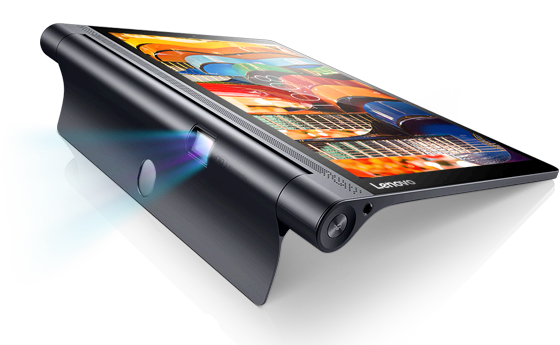
\includegraphics[width=0.38\linewidth]{Extra/lenovo_yoga_tab3_pro_front.png} 
  \caption{Moja prva slika}
  \label{slk:prvaslika}
\end{figure}

Referenciramo se na sliku \ref{slk:prvaslika} u sredini rečenice, zatim prije zareza \ref{slk:prvaslika}, te zatim na kraju rečenice \ref{slk:prvaslika}.
Upravo smo testirali radi li naredba \verb|\ref| ispravno u slučaju kada nakon nje slijedi točka.

Sada slijedi jedna jednadžba:
\begin{equation}
  \label{jed:prvajednadzba}
  \int_{-\infty}^{+\infty}f(t)\,dt=F(\omega)
\end{equation}
Jednadžba \eqref{jed:prvajednadzba} je moja prva jednadžba koja definira par $f(t)\ufrek F(\omega)$ ili $F(\omega)\uvrem f(t)$.

\cite{1980Axelrod1}
\cite{1980Axelrod2}
\cite{igraHrEnc}

\break

	Zatvorenikova dilema jedan je od najpoznatijih problema iz područja teorije igara. Dilema proučava interakciju između dvaju pojedinaca kroz igru suradnje i izdaje. Zatvorenikova dilema se može pronaći u korijenu mnogih interakcija koje se pojavljuju u društvu, ali i u životinjskom svijetu. Glavno pitanje je kako ta interakcija utječe na dobrobit oba igrača. Paradoks u Zatvorenikove dileme je činjenica da racionalno razmišljanje navodi svakog pojedinca da odabire opciju koja ne odgovara niti jednom od igrača \cite{PrisDilemmaHrEnc}.
	
	U stvarnom životu su takve interakcije često ponavljajuće prirode. Tada je potrebno imati na umu da će druga strana vjerojatno imati iskustvo prošlih interakcija što može utjecati na njihovu odluku u novoj interakciji. Stoga je interesantno razmatranje malo složenijeg problema iterirajuće Zatvorenikove dileme. Zanimljivo je da se u iterirajućem problemu mijenja pristup optimalnoj strategiji u odnosu na jednokratnu Zatvorenikovu dilemu.
	
	U korijenu Zatvorenikove dileme je napetost između individualnog racionalizma (u pogledu da je objema stranama smisleno biti sebičan) i grupnog racionalizma (objema stranama je isplativija obostrana suradnja nego obostrana izdaja) \cite{1980Axelrod1}.
	
	Mnogo je radova na pisano na temu optimalnog načina igranja Zatvorenikove dileme. Tako je Robert Axelrod iz Sveučilišta u Michiganu održao dva turnira u kojima su sudionici predavali svoje strategije za igranje igre u obliku računalnih programa \cite{1980Axelrod1} \cite{1980Axelrod2}. Analizom turnira došlo se zanimljivih zaključaka. Axelrod je proučavanjem strategija i njihovih rezultata izlučio nekoliko karakteristika koje imale tendenciju davati bolje rezultate. Te karakteristike su ljubaznost, opraštanje i provokabilnost \cite{1980Axelrod2}.
	
	Glavni cilj ovog rada je napraviti model inteligentnog igrača koji će naučiti igrati iterirajuću Zatvorenikovu dilemu. Cilj ovoga je proučiti kakvo će ponašanje razviti inteligentni igrač i kako će igrati protiv nekih drugih poznatih strategija. Također će biti zanimljivo analizirati ponašanje inteligentnog igrača i vidjeti je li razvio karakteristike koje su se pokazale poželjnima u Axelrodovim turnirima.

%-------------------------------------------------------------------------------
\chapter{Zatvorenikova dilema}
\label{pog:glavni_dio}

	Zatvorenikova dilema je poznati problem iz područja teorije igara koji proučava odnose između pojedinaca. Radi se o igri sa dva igrača koji imaju na izboru dva poteza: suradnja sa drugim igračem, ili izdaja drugog igrača. S obzirom na odabir oba igrača, svakom od njih se daje određena kazna ili nagrada. 
	
	Dilema je dobila naziv po ilustrativnom opisu Alberta Tuckera \cite{TeorijaIgaraIPravo}. Dilema je opisana u kontekstu odvojenog ispitivanja dvojice osumnjičenih kriminalaca. Svaki od osumnjičenih može priznati krivnju (ekvivalentno izdaji) ili šutjeti (ekvivalentno suradnji). Sukladno njihovim potezima dodjeljuju im se zatvorske kazne.
	
	Dilema se naravno može staviti i opisati kroz razne slikovite kontekste. No, u ovom radu ćemo radi jednostavnosti dilemu gledati samo kao igru u kojoj igrači skupljaju bodove.
	
	\textit{\textbf{Još raspisati?}}

	Generalna pravila za "bodovanje" je da obostrana suradnja i obostrana izdaja daju simetričnu podjelu bodova, uz to da suradnja daje veći broj bodova. U slučaju da jedan igrač surađuje dok ga drugi izdaje dolazi do nesimetrične podjele bodova. Igrač koje je izdan mora dobiti manje bodove nego bi dobio obostranom izdajom. Igrač koji ga je izdao tim potezom mora dobiti više nego bi dobio obostranom suradnjom. Tipična raspodjela bodova \cite{1980Axelrod1} koja će se koristiti i u ovom radu dana je u tablici \ref{Payoffs}.
	
	\break
	
	\begin{longtblr}[
		caption={Bodovanje odluka igrača u Zatvorenikovoj dilemi \\
				Napomena: Bodovi Igrača 1 su dani prvim brojem u svakom od parova.},
		label=Payoffs,
		entry=none
		]{
			width = \textwidth,
			colspec={|X[1,l]|X[2, l]|X[2, l]|X[2,l]|}, 
			rowhead = 0,
		} %definicija širine tablice, širine stupaca, poravnanje i broja redaka naslova tablice
		\hline 
		\SetCell[c=2, r=2]{c,r}{} & & \SetCell[c=2]{c}{Igrač 2} \\ \hline
	 & & Suradnja & Izdaja \\ \hline
 		\SetCell[r=2]{r}{Igrač 1} & Suradnja & 3, 3 & 0, 5 \\ \hline
	 & Izdaja & 5, 0 & 1, 1 \\ \hline
	\end{longtblr}
	 
	Važno je primijetiti da je Zatvorenikova dilema igra s promjenjivim ishodom \cite{PrisDilemmaHrEnc}. To znači da dobitak jednog igrača nije nužno gubitak drugog igrača i gubitak jednog igrača ne mora nužno biti dobitak drugog igrača \cite{igraHrEnc}. Drugim riječima, mogući su ishodi u kojima oba igrača profitiraju ili oba igrača gube. Upravo ova karakteristika omogućuje suradnji da bude poželjan pristup igranju. 
	 
	Zbog ove karakteristike Zatvorenikova dilema dobro opisuje mnoge probleme iz stvarnog života i objašnjava zašto je ponekad suradnja sa neprijateljem poželjna. Poznati je takav primjer problem prekomjernog naoružavanja i međusobnog nepovjerenja SAD-a i SSSR-a tijekom hladnog rata \cite{1980Axelrod1} Upravo je i taj problem bio jedan od motiva nastanka i proučavanja Zatvorenikove dileme.

	\section{Dobra strategija}
	
		Pitanje koje se prirodno nameće u Zatvorenikovoj dilemi je dosta očito: Kako dobro igrati ovu igru? Kojom strategijom pristupiti ovoj igri?

		U svrhu istraživanja optimalnih strategija Robert Axelrod je 1980. organizirao turnir \cite{1980Axelrod1} u koji je pozvao znanstvenike iz raznih područja koji su se bavili Zatvorenikovom dilemom. Učesnici su za turnir izradili strategije igranja Zatvorenikove dileme u obliku računalnog programa. Svaka strategija je igrala Zatvorenikovu dilemu u 200 iteracija sa svakom drugom strategijom, sa samom sobom i sa dodatnom strategijom koja je donosila nasumične odluke. Kasnije te godine Axelrod je organizirao još jedan sličan turnir u svrhu provođenja dodatne analize \cite{1980Axelrod2}.
	
		Pobjednik u oba turnira je bila strategija zvana "Tit for Tat", također poznata i kao "Copycat". Strategija je vrlo jednostavna. Na prvom potezu uvijek surađuje, a dalje uvijek kopira suparnikov prethodni potez \cite{1980Axelrod1}.
	
		Axelrod je analizom rezultata oba turnira pronašao nekoliko karakteristika koje su bile ključne za uspješnost strategija u oba turnira. Pronađene karakteristike su:
	
		\begin{itemize}
			\item \textbf{Ljubaznost} (eng. niceness) \cite{1980Axelrod1} - strategija je ljubazna ako nikada neće prva izdati drugog igrača
			\item \textbf{Sklonost opraštanju} (eng. forgiveness) \cite{1980Axelrod1} - sklonost strategije da surađuje nakon što ju je drugi igrač izdao
			\item \textbf{Provokabilnost} (eng. provocability) \cite{1980Axelrod2} - sklonost da strategija izda drugog igrača nakon što ju je drugi igrač izdao
		\end{itemize}
	
		Strategija "Tit for Tat" je bila uspješna jer je imala sve navedene karakteristike. "Tit for Tat" je ljubazna strategija jer počinje sa suradnjom i izdaje samo ako ju je drugi igrač izdao prvi. Strategija oprašta jer će nakon što bude jedom izdana uzvratiti izdajom, ali će nakon toga nastaviti surađivati dok ponovno ne bude izdana. Također, strategija je provokabilna jer će nakon što bude izdana uzvratiti izdajom.
	
		Axelrod je u svojem radu napomenuo važnu stvar, a to je da ne postoji najbolja strategija za Zatvorenikovu dilemu. To proizlazi iz jednostavne činjenice da performansa strategije uvelike ovisi o strategijama s kojima ta strategija igra. Dakle, okruženje u kojem se nalazi je od presudne važnosti \cite{1980Axelrod1}.
	
		No kroz detaljnu analizu drugog turnira Axelrod je ustanovio da su navedene karakteristike generalno poželjne i u pravilu donose dobre rezultate. Također, iako "Tit for Tat" nije univerzalno najbolja strategija, pokazuje se da generalno daje odlične rezultate u raznim okruženjima zbog dobro kombiniranih poželjnih karakteristika \cite{1980Axelrod2}.
	
		Axelrod je također napomenuo da je kod kreiranja strategije potrebna analiza na barem 3 dubine \cite{1980Axelrod1}. Prva razina je direktna posljedica trenutne odluke, to jest, koliko bodova igrač dobiva na temelju svoje odluke. Druga razina je uzimanje u obzira da će drugi igrač možda odlučiti kazniti izdaju. Treća razina razmatra da reagiranje na izdaju može prouzrokovati eho efekt međusobnih izdaja koji će dugoročno štetiti i jednom i drugom igraču.

\chapter{Umjetne neuronske mreže}

	U svrhu implementacije inteligentnog igrača koji će igrati Zatvorenikovu dilemu korištene su umjetne neuronske mreže.
	
	Umjetne neuronske mreže su jedan od mnogih koncepata u strojnom učenju, koje je najpopularnija grana područja umjetne inteligencije. Neuronsku mrežu čine međusobno povezani umjetni neuroni. Područje koje se bavi umjetnim neuronskim mrežama zove se neuro-računarstvo, koje čini granu računarstva iz skupine mekog-računarstva. \cite{skriptaNeuronskeMreze} 
	
	Umjetni neuron je najmanja funkcionalna jedinka neuronske mreže i modelira biološki neuron u ljudskom mozgu. Umjetni neuroni imaju ulogu jednostavne procesne jedinice. Svaki umjetni neuron na ulazu prima nekakve vrijednosti (izlazi drugih neurona ili ulazni podaci). Dobiveni ulazi se zbrajaju u jednu sumu koja se provlači kroz takozvanu prijenosnu funkciju. Rezultat prijenosne funkcije se postavlja na izlaz umjetnog neurona te se propagira dalje na ulaze drugih neurona ili na izlaz neuronske mreže. Postoje razne prijenosne funkcije različitih složenosti koje se mogu koristiti kod umjetnih neurona, a neke od njih su: funkcija identiteta, funkcija skoka, sigmoidna funkcija, tangens hiperbolni, funkcija zglobnica, funkcija propusna zglobnica \cite{skriptaNeuronskeMreze}.

	\textit{\textbf{Neka slika neurona (i prijenosnih funkcija)}}
	
	Arhitektura umjetne neuronske mreže opisuje kako su povezani umjetni neuroni u mreži i koliko ih ima. Postoje razne arhitekture neuronskih mreža, što jednostavnih, što kompleksnih, a svaka ima svoje prednosti i područja u kojima su našle primjenu. Neke od generalnih vrsta umjetnih neuronskih mreža su unaprijedna, povratna, potpuno povezana, konvolucijska.
	
	Umjetni neuroni se u umjetnim neuronskim mrežama obično organiziraju u slojeve. Tako razlikujemo ulazni sloj, skrivene slojeve i izlazni sloj. Skriveni slojevi i izlazni sloj se sastoje od umjetnih neurona dok ulazni sloj zapravo ne sadrži umjetne neurone kakvi su opisani u odjeljku iznad. Neuroni ulaznog sloja na svoje ulaze samo primaju ulazne podatke neuronske mreže te ih dalje prosljeđuju neuronima prvog skrivenog sloja.
	
	Umjetne neuronske mreže danas imaju vrlo široku primjenu, od obrade slika i signala, prepoznavanja uzoraka, kompresije slika, upravljanja, financija... \cite{skriptaNeuronskeMreze}. Glavne prednosti neuronskih mreža su vrlo dobra sposobnost generalizacije i učenja, dok im je glavna mana nemogućnost interpretacije njihovog ponašanja. Slično kao i kod ljudskog mozga, teško je razumjeti zašto je neuronska mreža za neki ulaz dala baš taj izraz. Također, još je teže prepoznati kakvu je konkretnu ulogu u sveukupnoj obradi ulaza imao pojedini neuron u mreži.
	
	U ovom radu koristit će se potpuno povezana Elmanova neuronska mreža \textit{\textbf{točno???}}. Kod potpuno povezane mreže svaki neuron ima vezu prema svakom neuronu iz slijedećeg sloja. 
	
	\section{Elmanova neuronska mreža}
	
		Elmanova neuronska mreža je jednostavna povratna neuronska mreža (\textit{eng. Recurrent Neural Network}). Glavna karakteristika takvih mreža je da imaju neku vrstu povratne veze ili vremenski odgođene veze \cite{ElmanNetSite}.
		
		Elmanova neuronska mreža se sastoji od ulaznog sloja, jednog skrivenog sloja i izlaznog sloja. Skriveni sloj ove mreže dodatno ima skriveni kontekst. Kontekst čine neuroni koji služe za pohranu kontekstnih podataka. Dodatno postoje veze iz izlaza skrivenog sloja prema kontekstu i veze iz konteksta prema ulazu u skriveni sloj. Izlaz iz skrivenog sloja se preko tih veza sprema u kontekst. Kod obrade sljedećeg ulaza u neuronsku mrežu u skrivenom se sloju vrijednosti iz konteksta pribrajaju međurezultatu obrade prije primjene prijenosne funkcije.
		
		\textit{\textbf{Neka slika Elmanove mreže}}
		
		Ovime se omogućava da Elmanova mreža može pamtiti prošla stanja. na ovaj način prijašnji ulazi u neuronsku mrežu utječu na rezultat obrade nekog budućeg ulaza.
		
		Ovo je korisno svojstvo za model inteligentnog igrača Zatvorenikove dileme, s obzirom da je prirodno da prijašnje interakcije sa drugim igračem utječu na nove odluke.
	
\chapter{Evolucijsko računanje}

	Evolucijsko računanje je grana umjetne inteligencije koja se najčešće bavi rješavanjem optimizacijskih problema. Začeci ove grane sežu još u kasne 50-te godine prošlog stoljeća. Evolucijsko računanje se može podijeliti u tri grane \cite{skriptaEvolucijskoRacunarstvo}: 
	\begin{itemize}
		\item \textit{evolucijske algoritme}
		\item \textit{algoritme rojeva}
		\item \textit{ostale algoritme}
	\end{itemize}
	
	Neki od algoritama iz grane evolucijskih algoritama su evolucijske strategije, evolucijsko programiranje, genetski algoritam i genetsko programiranje \cite{skriptaEvolucijskoRacunarstvo}.
	
	U grani algoritma rojeva nalaze se mravlji algoritmi, algoritam roja čestica, algoritmi pčela i drugi \cite{skriptaEvolucijskoRacunarstvo}.
	
	Neki do značajnih algoritama iz grane ostali algoritmi pripadaju umjetni imunološki algoritmi, algoritam diferencijske evolucije i algoritam harmonijske pretrage \cite{skriptaEvolucijskoRacunarstvo}.
	
	Područje evolucijskog računanja također pripada području metaheuristika. Metaheuristika je skup algoritamskih koncepata koji se koriste za definiranje heurističkih metoda primjenjivih na široki skup problema \cite{skriptaEvolucijskoRacunarstvo}. Heurističke metode su algoritmi koji pronalaze rješenja problema koja su zadovoljavajuće dobra, ali ne nužno optimalna. Heurističke metode obično imaju relativnu nisku računsku složenost \cite{skriptaEvolucijskoRacunarstvo}.

	\section{Optimizacija}
	
		Kao što je ranije navedeno, algoritmi iz područja evolucijskog računanja se često koriste u problemima optimizacije. Optimizaciju možemo definirati kao postupak pronalaženja najboljeg rješenja problema. Uz svako rješenje se pridružuje funkcija dobrote ili funkcija kazne. Ako se rješenjima pridružuje funkcija dobrote, optimizacijski postupak će tražiti rješenje tako da pokuša maksimizirati funkciju dobrote. Ako se pak rješenjima pridružuje funkcija kazne, optimizacijski postupak će pokušati minimizirati funkciju kazne \cite{skriptaEvolucijskoRacunarstvo}.

		Bitno je reći da kada gledamo optimizacijske algoritme iz područja evolucijskog računanja, niti jedan od njih se ne može istaknuti kao generalno najbolji algoritam. Svaki od tih algoritama je dobar u određenim primjenama, dok u drugim primjenama drugi optimizacijski algoritmi daju bolje rezultate. U prosjeku nema značajnih razlika u globalnim performansama kada se gleda prosjek po svim mogućim funkcijama cijene \cite{skriptaEvolucijskoRacunarstvo}.
	
	\section{Genetski algoritam}
	
		
	
	
\chapter{Definiranje pokusa}

	Jedna "iteracija" se sastoji od npr. 50 ponavljanja Zatvorenikove dileme.


% \Blindtext


%-------------------------------------------------------------------------------
\chapter{Rezultati i rasprava}
\label{pog:rezultati_i_rasprava}

% \Blindtext


%--- ZAKLJUČAK / CONCLUSION ----------------------------------------------------
\chapter{Zaključak}
\label{pog:zakljucak}

Na kraju rada piše se kratak zaključak, duljine do najviše jedne stranice. 
% \blindtext


%--- LITERATURA / REFERENCES ---------------------------------------------------

% Literatura se automatski generira iz zadane .bib datoteke / References are automatically generated from the supplied .bib file
% Upiši ime BibTeX datoteke bez .bib nastavka / Enter the name of the BibTeX file without .bib extension
\bibliography{literatura}



%--- SAŽETAK / ABSTRACT --------------------------------------------------------

% Sažetak na hrvatskom
\begin{sazetak}
  Unesite sažetak na hrvatskom.

	Naslov, sažetak, ključne riječi (na hrvatskom jeziku)
	Sažetak opisuje sadržaj rada, prepričan u stotinjak riječi. 

  % \blindtext
\end{sazetak}

\begin{kljucnerijeci}
	Zatvorenikova dilema, umjetna inteligencija, umjetne neuronske mreže, inteligentni igrač
\end{kljucnerijeci}


% Abstract in English
\begin{abstract}
  Enter the abstract in English.
  
  Title, summary, keywords (na engleskom jeziku)
  
  % \blindtext 
\end{abstract}

\begin{keywords}
  Prisoner's dilemma, Artificial intelligence, Artificial neural networks, Intelligent player
\end{keywords}


%--- PRIVITCI / APPENDIX -------------------------------------------------------

% Sva poglavlja koja slijede će biti označena slovom i riječi privitak / All following chapters will be denoted with an appendix and a letter
\backmatter

\chapter{The Code}

	Privitak je također opcionalno poglavlje (u dogovoru s mentorom). 
	Sadržaj koji se stavlja u privitak je, općenito, nešto što je, kao cjelinu, prikladno izdvojiti iz sadržaja samog rada.
	Mogući primjer je tehnička dokumentacija vezana uz završni rad - npr. električka i položajna shema sklopa, sastavnica, predložak tiskane veze, plan bušenja, ispis programa s detaljnim opisom.
	Drugi primjer uključuju upute za korištenje rezultata rada (softvera ili hardvera), detaljni ispisi mjerenja čiji su rezultati sažeto ili grafički prikazani u radu. Ako se radi o softveru, uobičajeno je navesti podatke o platformi na kojoj se izvodi (npr., karakteristike uređaja i operacijskog sustava te pomoćnog softvera), kao i upute za instalaciju. 
	
	U privitku nemojte koristiti stilove razine Heading, već samo (nenumerirani) stil Podnaslov. 
	Na primjer:
	
	Instalacija programske podrške
	
	Upute za korištenje programske podrške


% \Blindtext


\end{document}
